% *********************************************************************
% © 2010–2026 Jeremy Sylvestre
%
% Permission is granted to copy, distribute and/or modify this document
% under the terms of the GNU Free Documentation License, Version 1.3 or
% any later version published by the Free Software Foundation; with no
% Invariant Sections, no Front-Cover Texts, and no Back-Cover Texts. A
% copy of the license is included in the appendix entitled “GNU Free
% Documentation License” that appears in the output document of this
% PreTeXt source code. All trademarks™ are the registered® marks of
% their respective owners.
%
% *********************************************************************

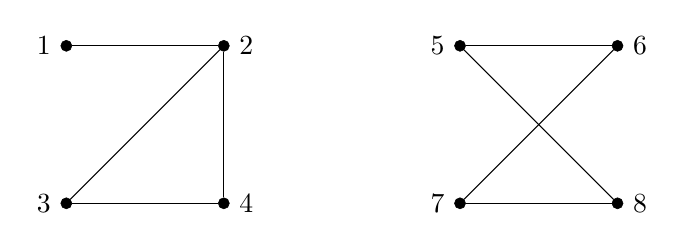
\begin{tikzpicture}[
	vertex/.style={ circle, draw, very thin, fill, inner sep=0pt, minimum size=4pt },
	vertexg/.style={ black!40!white, circle, draw, very thin, fill, inner sep=0pt, minimum size=4pt },
	vertexo/.style={ circle, draw, very thin, inner sep=0pt, minimum size=4pt }
]

\node at (0,0) (v3) [vertex,label=left:$3$] {};
\node at (2,0) (v4) [vertex,label=right:$4$] {};
\draw (v3) to (v4);
\node at (2,2) (v2) [vertex,label=right:$2$] {};
\foreach \p in {v3,v4} \draw (\p) to (v2);
\node at (0,2) (v1) [vertex,label=left:$1$] {};
\draw (v2) to (v1);

\begin{scope}[xshift=5cm]
	\node at (0,0) (v3) [vertex,label=left:$7$] {};
	\node at (2,0) (v4) [vertex,label=right:$8$] {};
	\draw (v3) to (v4);
	\node at (2,2) (v2) [vertex,label=right:$6$] {};
	\draw (v3) to (v2);
	\node at (0,2) (v1) [vertex,label=left:$5$] {};
	\foreach \p in {v2,v4} \draw (\p) to (v1);
\end{scope}

\end{tikzpicture}
